\FILE{cc.tex}

\section{Hybrid Multi-Cloud Analytics Services
Framework}\label{hybrid-multi-cloud-analytics-services-framework}

\textbf{Cloudmesh Controlled Computing through Workflows}


\subsection{Background}\label{background}

High-performance computing (HPC) has been, for decades, a very important tool
for science. Scientific tasks can leverage the processing power of
a supercomputer so they can run at previously unobtainable high speeds
or utilize specialized hardware for acceleration that otherwise are not
available to the user. HPC can be used for analytic programs that
leverage machine learning applied to large data sets to, for example,
predict future values or to model current states. For such
high-complexity projects, there are often multiple complex programs that
may be running repeatedly in either competition or cooperation.
Leveraging computational GPUs, for instance, leads to several times higher
performance when applied to deep learning algorithms. With such
projects, program execution is submitted as a job to a typically remote
HPC center, where time is billed as node hours. Such projects must have
a service that lets the user manage and execute without supervision. We
have created a service that lets the user run jobs across multiple
platforms in a dynamic queue with visualization and data storage.

See \ref{fig:fastapi-service}.

\begin{figure}
\centering
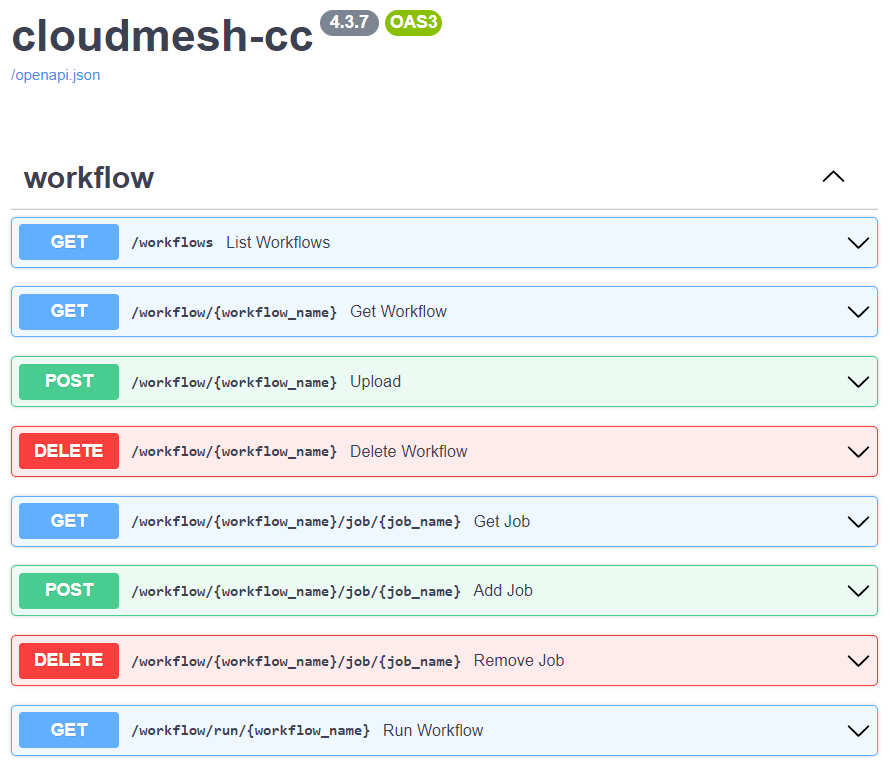
\includegraphics[width=1.0\columnwidth]{images/fastapi-service.png}
\caption{OpenAPI Description of the REST Interface to the
Workflow}\label{fig:fastapi-service}
\end{figure}

\subsection{Workflow Controlled
Computing}\label{workflow-controlled-computing}

This software was developed end enhancing Cloudmesh, a suite of software
to make using cloud and HPC resources easier. Specifically, we have
added a library called Cloudmesh Controlled Computing (cloudmesh-cc)
that adds workflow features to control the execution of jobs on remote
compute resources.

The goal is to provide numerous methods of specifying the workflows on a
local computer and running them on remote services such as HPC and cloud
computing resources. This includes REST services and command line tools.
The software developed is freely available and can easily be installed
with standard Python tools so integration in the Python ecosystem using
virtualenv's and Anaconda is simple.


\subsection{Workflow Functionality}\label{workflow-functionality}

A hybrid multi-cloud analytics service framework was created to manage
heterogeneous and remote workflows, queues, and jobs. It was designed
for access through both the command line and REST services to simplify
the coordination of tasks on remote computers. In addition, this service
supports multiple operating systems like macOS, Linux, and Windows 10
and 11, on various hosts: the computer's localhost, remote computers,
and the Linux-based virtual image WSL. Jobs can be visualized and saved
as a YAML and SVG data file. This workflow was extensively tested for
functionality and reproducibility.

\subsection{Quickstart}\label{quickstart}

To test the workflow program, prepare a cm directory in your home
directory by executing the following commands in a terminal:

\bigbreak
\begin{minted}[breaklines]{bash}
$ mkdir ~/cm
$ cd ~/cm
$ pip install cloudmesh-installer -U
$ cloudmesh-installer get cc
$ cd cloudmesh-cc
$ pytest -v -x --capture=no tests/test_199_workflow_clean.py
\end{minted}
\bigbreak

This test runs three jobs within a singular workflow: the first job runs
a local shell script, the second runs a local Python script, and the
third runs a local Jupyter notebook.

\subsection{Application demonstration using
MNIST}\label{application-demonstration-using-mnist}

The Modified National Institute of Standards and Technology Database is
a machine learning database based on image processing. Various MNIST
files involving different machine learning cases were modified and
tested on various local and remote machines. These cases include
Multilayer Perceptron, LSTM (Long short-term memory), Auto-Encoder,
Convolutional, and Recurrent Neural Networks, Distributed Training, and
PyTorch training.

See Table \ref{table:mnist-times} for benchmarks of the MNIST workflow
on UVA's supercomputer, Rivanna.

\begin{figure}
\centering
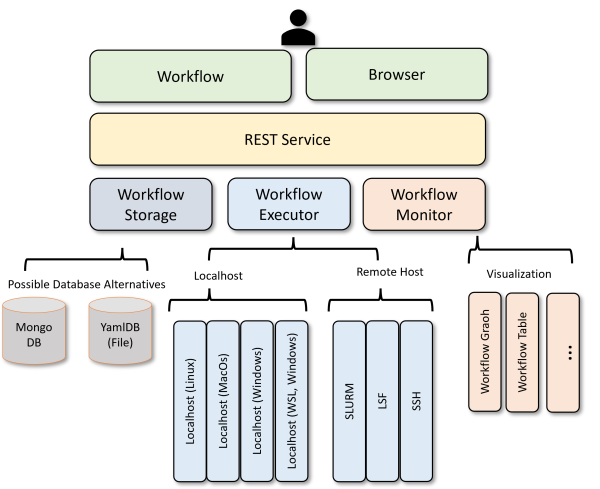
\includegraphics[width=1.0\columnwidth]{images/workflow-uml.png}
\caption{Design for the workflow.}\label{fig:workflow-uml}
\end{figure}

\subsection{Design}\label{design}

The hybrid multi-cloud analytics service framework was created to ensure
running jobs across many platforms. We designed a small and streamlined
number of abstractions so that jobs and workflows can be represented
easily. The design is flexible and can be expanded as each job can
contain arbitrary arguments. This made it possible to custom design for
each target type a specific job type so that execution on local and
remote compute resources including batch operating systems can be
achieved. The job types supported include: local job on Linux, macOS,
Windows 10, and Windows 11, jobs running in WSL on Windows computers,
remote jobs using ssh, and batch jobs using Slurm.

In addition, we leveraged the existing Networkx Graph framework to allow
dependencies between jobs. This greatly reduced the complexity of the
implementation while being able to leverage graphical displays of the
workflow, as well as using scheduling jobs with for example topological
sort available in Networkx. Custom schedulers can be designed easily
based on the dependencies and job types managed through this
straightforward interface. The status of the jobs is stored in a
database that can be monitored during program execution. The creation of
the jobs is done on the fly, e.g.~when the job is needed to be
determined on the dependencies when all its parents are resolved. This
is especially important as it allows dynamic workflow patterns to be
implemented while results from previous calculations can be used in
later stages of the workflow.

We have developed a simple-to-use API for this so programs can be
formulated using the API in Python. However, we also embedded this API
in a prototype REST service to showcase that integration into
language-independent frameworks is possible. The obvious functions to
manage workflows are supported including graph specification through
configuration files, upload of workflows, export, adding jobs and
dependencies, and visualizing the workflow during the execution. An
important feature that we added is the monitoring of the jobs while
using progress reports through automated log file mining. This way each
job reports the progress during the execution. This is especially of
importance when we run very complex and long-running jobs.

The REST service was implemented in FastAPI to leverage a small but fast
service that features a much smaller footprint for implementation and
setup in contrast to other similar REST service frameworks using Python.

This architectural component building this framework is depicted
@fig:workflow-uml. The code is available in this repository and manual
pages are provided on how to install it:
\href{https://github.com/cloudmesh/cloudmesh-cc}{cloudmesh-cc}.

\subsection{Summary}\label{summary}

The main interaction with the workflow is through the command line. With
the framework, researchers and scientists should be able to create jobs
on their own, place them in the workflow, and run them on various types
of computers.

In addition, developers and users can utilize the built-in OpenAPI
graphical user interface to manage workflows between jobs. They can be
uploaded as YAML files or individually added through the build-in debug
framework.

Improvements to this project will include code cleanup and manual
development.

\subsection{References}\label{references}

A poster based on a pre-alpha version of this code is available as ppt
and PDF file. However, that version is no longer valid and is superseded
by much improved efforts. The code summarized in the pre-alpha version
was mainly used to teach a number of students Python and how to work in
a team.

\begin{itemize}
\item
  \href{https://github.com/cloudmesh/cloudmesh-cc/raw/main/documents/analytics-service.pptx}{Poster
  Presentation (PPTX)}
\item
  \href{https://github.com/cloudmesh/cloudmesh-cc/raw/main/documents/analytics-service.pdf}{Poster
  Presentation (PDF)}
\end{itemize}

Please note also that the poster contains inaccurate statements and
descriptions and should not be used as a reference to this work.

